\documentclass{article}
\usepackage{tikz}
\usepackage[margin=1in]{geometry}
\usepackage{amsmath}
\begin{document}

\vfill
\begin{center}


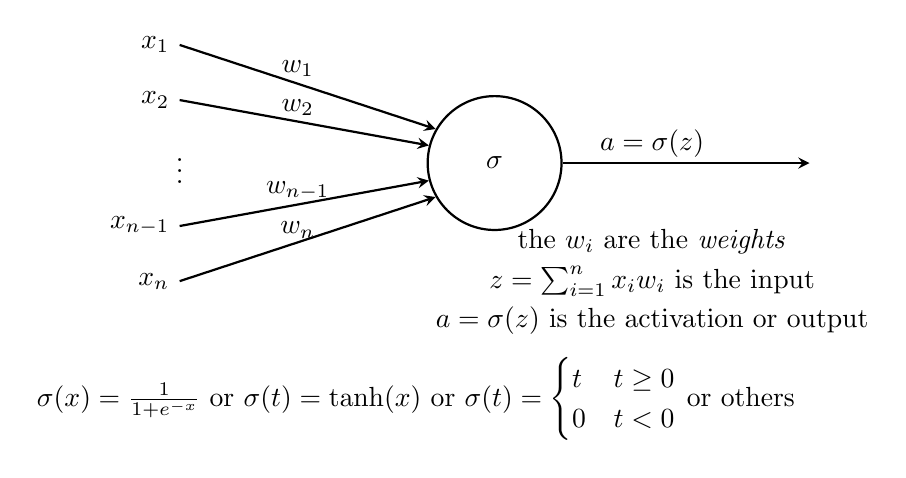
\begin{tikzpicture}[>=stealth,thick]

% Neuron node with sigma
\node[circle,draw,minimum size=1.7cm] (neuron) {$\sigma$};

% ---- Input arrows ----
% x1
\node[left] at (-4,1.5) {$x_1$};
\draw[->] (-4,1.5) -- (neuron.150);

% x2
\node[left] at (-4,0.8) {$x_2$};
\draw[->] (-4,0.8) -- (neuron.165);

% Ellipsis
\node at (-4,0) {$\vdots$};

% x_{n-1}
\node[left] at (-4,-0.8) {$x_{n-1}$};
\draw[->] (-4,-0.8) -- (neuron.195);

% x_n
\node[left] at (-4,-1.5) {$x_n$};
\draw[->] (-4,-1.5) -- (neuron.210);
\node at (2,.25) {$a=\sigma(z)$};

% ---- Weights (positioned as requested) ----
\node at (-2.5,1.2) {$w_1$};          % above first arrow
\node at (-2.5,.7) {$w_2$};         % between first and second

\node at (-2.5,-0.35) {$w_{n-1}$};     % just above third arrow
\node at (-2.5,-.85) {$w_n$};        % between third and fourth

% ---- Output ----
\draw[->] (neuron) -- (4,0);
\node at (2,-1) {the $w_{i}$ are the \emph{weights}};
\node at (2,-1.5) {$z=\sum_{i=1}^{n} x_{i}w_{i}$ is the input};
\node at (2, -2.0) {$a=\sigma(z)$ is the activation or output};

\node at (-1,-3.0) {$\sigma(x) = \frac{1}{1+e^{-x}}$ or $\sigma(t)=\tanh(x)$ or $\sigma(t)=\begin{cases} t & t\ge 0 \\ 0 & t<0\end{cases}$ or others};


\end{tikzpicture}
\end{center}
\vfill

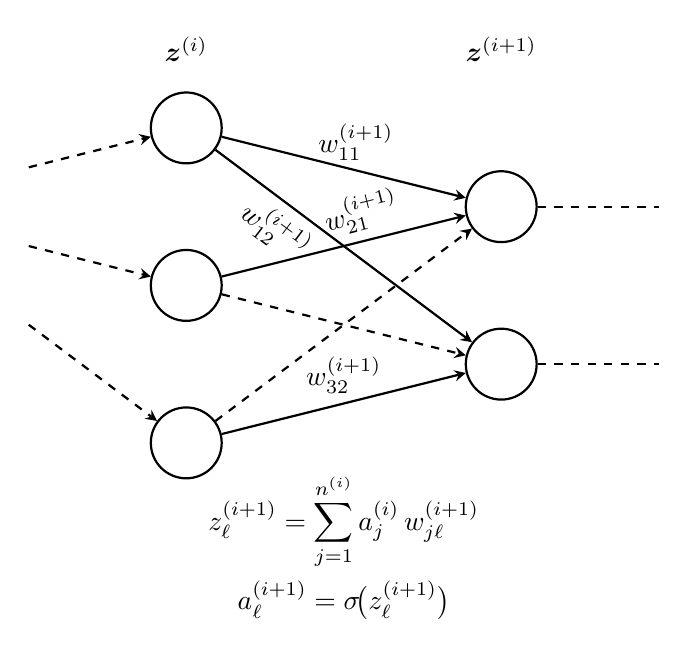
\begin{tikzpicture}[>=stealth,thick]

% ------------------------------------------------------------------
% Layer labels at the top
% ------------------------------------------------------------------
\node at (-2,3) {$\boldsymbol{z}^{(i)}$};
\node at ( 2,3) {$\boldsymbol{z}^{(i+1)}$};

% ------------------------------------------------------------------
% Neurons (layer i on the left, layer i+1 on the right)
% ------------------------------------------------------------------
\node[circle,draw,minimum size=0.9cm] (L1) at (-2, 2.0) {};
\node[circle,draw,minimum size=0.9cm] (L2) at (-2, 0.0) {};
\node[circle,draw,minimum size=0.9cm] (L3) at (-2,-2.0) {};

\node[circle,draw,minimum size=0.9cm] (R1) at ( 2, 1) {};
\node[circle,draw,minimum size=0.9cm] (R2) at ( 2,-1) {};

% ------------------------------------------------------------------
% Dashed connections from the rest of the network (left side)
% ------------------------------------------------------------------
\draw[dashed,->] (-4, 1.5) -- (L1);
\draw[dashed,->] (-4, 0.5) -- (L2);
\draw[dashed,->] (-4,-0.5) -- (L3);
\draw[dashed,->] (L2) -- (R2);
\draw[dashed,->] (L3) -- (R1) ; 

% ------------------------------------------------------------------
% Solid connections between the two layers with weight labels
% ------------------------------------------------------------------
\draw[->] (L1) -- (R1)
  node[pos=.55,above] {$w_{11}^{(i+1)}$};

\draw[->] (L2) -- (R1)
  node[pos=.6,above,sloped] {$w_{21}^{(i+1)}$};

\draw[->] (L1) -- (R2)
  node[pos=.3,below,sloped] {$w_{12}^{(i+1)}$};

\draw[->] (L3) -- (R2)
  node[midway,above] {$w_{32}^{(i+1)}$};

% ------------------------------------------------------------------
% Dashed outgoing connections to later layers (right side)
% ------------------------------------------------------------------
\draw[dashed] (R1) -- ( 4, 1.0);
\draw[dashed] (R2) -- ( 4,-1.0);

% ------------------------------------------------------------------
% Formulas underneath
% ------------------------------------------------------------------
\node at (0,-3)
  {$z_\ell^{(i+1)} = \displaystyle\sum_{j=1}^{n^{(i)}} a_j^{(i)}\,w_{j\ell}^{(i+1)}$};

\node at (0,-4)
  {$a_\ell^{(i+1)} = \sigma\!\bigl(z_\ell^{(i+1)}\bigr)$};

\end{tikzpicture}



\end{document}